% \documentclass{article}
% \usepackage[utf8]{inputenc}
% \usepackage{amsmath}
%
% \title{Lecture 01: Graphs}
% \author{the writer}
% \date {30/09/2025}
% \begin{document}
% \maketitle
% \section{Finite graph:}
% \section{directed graph:}
% \section{Successor and precssor graph:}
% \section{cardinality of vertices and arcs/edges:}
% in a finite graph G = (V,E) defined by the finite set of \textbf{edges} 
%
%  $E = \left\{ e1, e2, e3 ,e4, e5 \right\} $ 
% \section {Degree of a vertex (vertx degree) }
% \section {Chain vs Path}
%
% \subsection {(chain) == undirected graph }
% elementary chain vs simple chain
%
% elementary chain cannot visit the same vertex twice. \\
% A simple chain cannot vist the same edge twice 
%
% a chain can be both simple and elementary
%
% \subsection {Path(path) == directed graph}
%
% elementary path vs simple path
%
% \subsection {circuit}
% A circuit is a simple closed path  ( \textbf{the directions matters})
% \\A \textit{cycle} is same as circuit but \textbf{directions doesn't matter }
%
% \subsection{complete graph}
%
% if all pairs are adjacent
% subsection{Tournament (complete drected graph}
%
% \subsection{simple graph}
% A finite graph G = (V,E) os said to be \textbf{simple}, if it does not contain a loop and there is \\
% no  more  than one edge connecting two same vertices
%
% \subsection{Multigraph}
%
% A finite graph G = (V,E) is called a\\
% multigraph if it contains loops\\
% and/or multiple edges connecting the same vertices.
%
% \subsection{SubGraph}
% an \textbf{Induced subgraph} is obtained by 
% removing from a graph vertices and all edges incedent 
% to those vertices
%
% \subsection{Partial graph(spanning subgraph)}
%
% A partial graph (spanning subraph) is obtained by removin edger from a graph
%
% \subsection{Eulerian graph/pat/chain/circuit/cycle}
% A chain or cycle is said to be Eulerian if each edge of the graph appears exactly once. 
% Paths and circuits of digraphs are said to be 
% Eulerian under the same conditions.
% A graph/digraph is said to be Eulerian if it admits and Eulerian cycle/circuit.
%
% \subsection{Hamiltonian graph/path/chain/circuit/cycle)}
% A cahin or cycle is said to be Hamiltonian if each vertex of 
% the graph appears exactly once. Paths and circuits of digraphs are said to be Hamiltonian under the same conditions.\\
% A graph/digraph is said to be Hamiltonian if it admits a Hamiltonian cycle/circuit.
%
% \subsection{Tree}
% A \textbf{tree} is a connected graph containing no cycles.
%
% \subsection{Covering tree(spanning tree)}
% A covering tree (\textbf{Spanning tree}) is a maximal subgraph of a graph 
% containing non cycles (which is also a tree)
%
% \subsection{Rooted tree}
%
% A \textbf{Rooted tree} is a tree with a distinguished or favored top r(\textbf{Root}).
%
% \subsection{Forest}
% A \textbf{Forest} is a set of trees.
% A forest is a graph that does not contain cycles.
% The related componoents of the forest aree trees. 
%
%
%
% \end{document}

\documentclass{article}
\usepackage{amsmath}
\usepackage{tikz}
\usetikzlibrary{arrows}

\title{Lecture 01: Graphs}
\author{the writer}
\date{30/09/2025}

\begin{document}
\maketitle

\sloppy 
\section{Finite graph}
A finite graph $G = (V,E)$ defined by the finite set of \textbf{edges} 
$E = \{ e_1, e_2, e_3, e_4, e_5 \}$. 

\begin{center}
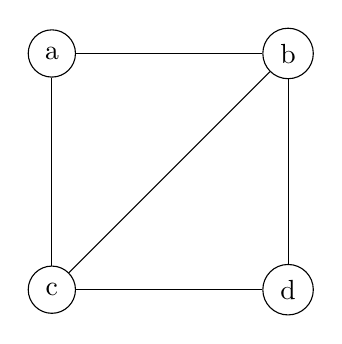
\begin{tikzpicture}[every node/.style={circle,draw,minimum size=6mm}]
  \node (a) {a};
  \node (b) [right of=a,xshift=2cm] {b};
  \node (c) [below of=a,yshift=-2cm] {c};
  \node (d) [right of=c,xshift=2cm] {d};
  \draw (a)--(b);
  \draw (a)--(c);
  \draw (b)--(d);
  \draw (c)--(d);
  \draw (b)--(c);
\end{tikzpicture}
\end{center}

\section{Directed graph}
\begin{center}
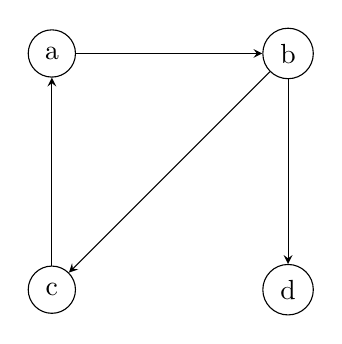
\begin{tikzpicture}[->,>=stealth,every node/.style={circle,draw,minimum size=6mm}]
  \node (a) {a};
  \node (b) [right of=a,xshift=2cm] {b};
  \node (c) [below of=a,yshift=-2cm] {c};
  \node (d) [right of=c,xshift=2cm] {d};
  \draw (a)--(b);
  \draw (b)--(c);
  \draw (c)--(a);
  \draw (b)--(d);
\end{tikzpicture}
\end{center}

\section{Simple graph}
A finite graph $G = (V,E)$ is said to be \textbf{simple}, if it does not contain a loop and there is 
no more than one edge connecting two same vertices.

\begin{center}
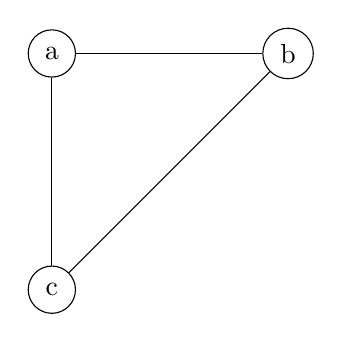
\begin{tikzpicture}[every node/.style={circle,draw,minimum size=6mm}]
  \node (a) {a};
  \node (b) [right of=a,xshift=2cm] {b};
  \node (c) [below of=a,yshift=-2cm] {c};
  \draw (a)--(b);
  \draw (b)--(c);
  \draw (c)--(a);
\end{tikzpicture}
\end{center}

\section{Multigraph}
A finite graph $G = (V,E)$ is called a multigraph if it contains loops
and/or multiple edges connecting the same vertices.

\begin{center}
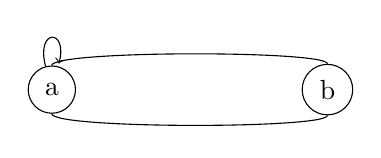
\begin{tikzpicture}[every node/.style={circle,draw,minimum size=6mm}]
  \node (a) {a};
  \node (b) [right of=a,xshift=2.5cm] {b};
  % Multiple edges
  \draw (a)..controls +(0,0.5) and +(0,0.5)..(b);
  \draw (a)..controls +(0,-0.5) and +(0,-0.5)..(b);
  % Loop
  \draw (a) edge[loop above] ();
\end{tikzpicture}
\end{center}

\section{Cycle / Circuit}
A circuit is a simple closed path (the directions matter). 
A \textit{cycle} is the same as a circuit but directions do not matter.

\begin{center}
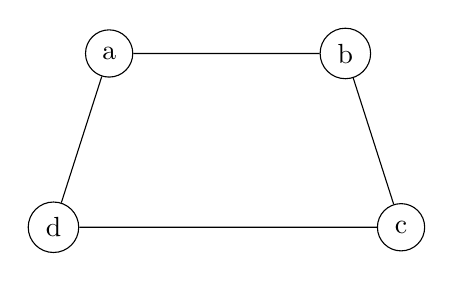
\begin{tikzpicture}[every node/.style={circle,draw,minimum size=6mm}]
  \node (a) {a};
  \node (b) [right of=a,xshift=2cm] {b};
  \node (c) [below right of=b,yshift=-1.5cm] {c};
  \node (d) [below left of=a,yshift=-1.5cm] {d};
  \draw (a)--(b)--(c)--(d)--(a);
\end{tikzpicture}
\end{center}

\section{Complete graph}
If all pairs are adjacent. Example $K_4$:

\begin{center}
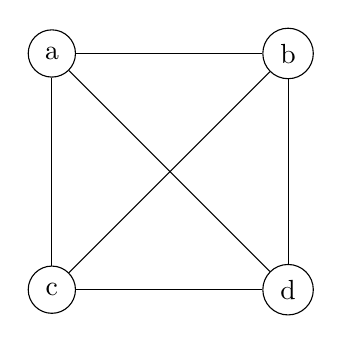
\begin{tikzpicture}[every node/.style={circle,draw,minimum size=6mm}]
  \node (a) {a};
  \node (b) [right of=a,xshift=2cm] {b};
  \node (c) [below of=a,yshift=-2cm] {c};
  \node (d) [below of=b,yshift=-2cm] {d};
  \foreach \i/\j in {a/b,a/c,a/d,b/c,b/d,c/d}
    \draw (\i)--(\j);
\end{tikzpicture}
\end{center}

\section{Tournament (complete directed graph)}
\begin{center}
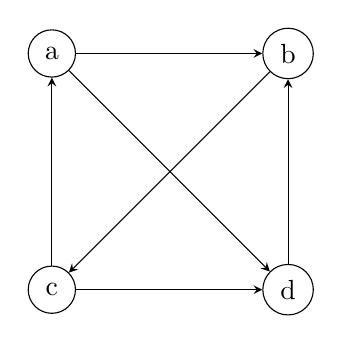
\begin{tikzpicture}[->,>=stealth,every node/.style={circle,draw,minimum size=6mm}]
  \node (a) {a};
  \node (b) [right of=a,xshift=2cm] {b};
  \node (c) [below of=a,yshift=-2cm] {c};
  \node (d) [below of=b,yshift=-2cm] {d};
  \draw (a)->(b);
  \draw (b)->(c);
  \draw (c)->(a);
  \draw (a)->(d);
  \draw (d)->(b);
  \draw (c)->(d);
\end{tikzpicture}
\end{center}

\section{Eulerian graph / path / circuit}
A chain or cycle is said to be Eulerian if each edge of the graph appears exactly once. 
A graph/digraph is Eulerian if it admits an Eulerian cycle/circuit.

\begin{center}
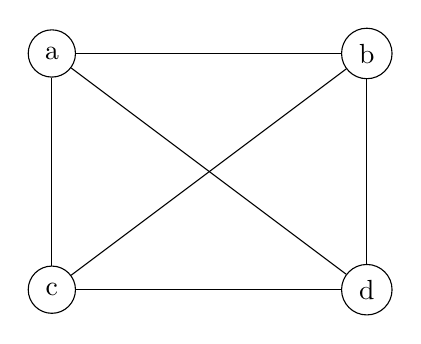
\begin{tikzpicture}[every node/.style={circle,draw,minimum size=6mm}]
  \node (a) {a};
  \node (b) [right of=a,xshift=3cm] {b};
  \node (c) [below of=a,yshift=-2cm] {c};
  \node (d) [below of=b,yshift=-2cm] {d};
  \draw (a)--(b)--(d)--(c)--(a);
  \draw (a)--(d);
  \draw (b)--(c);
\end{tikzpicture}
\end{center}

\section{Hamiltonian graph / path / cycle}
A chain or cycle is said to be Hamiltonian if each vertex of 
the graph appears exactly once. 
A graph/digraph is Hamiltonian if it admits a Hamiltonian cycle/circuit.

\begin{center}
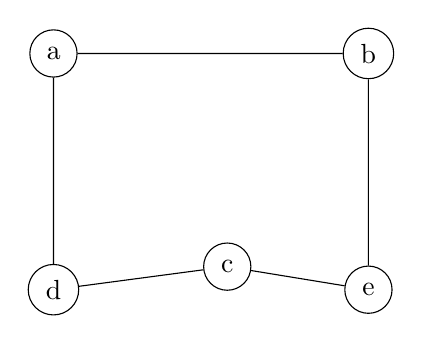
\begin{tikzpicture}[every node/.style={circle,draw,minimum size=6mm}]
  \node (a) {a};
  \node (b) [right of=a,xshift=3cm] {b};
  \node (c) [below right of=a,xshift=1.5cm,yshift=-2cm] {c};
  \node (d) [below of=a,yshift=-2cm] {d};
  \node (e) [below of=b,yshift=-2cm] {e};
  % Hamiltonian cycle visiting each vertex once
  \draw (a)--(b)--(e)--(c)--(d)--(a);
\end{tikzpicture}
\end{center}

\section{Tree}
A \textbf{tree} is a connected graph containing no cycles.

\begin{center}
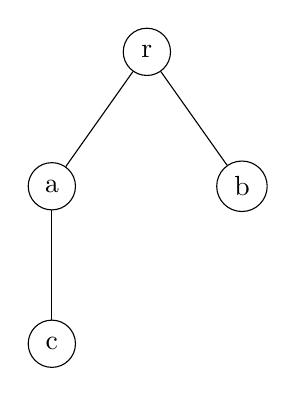
\begin{tikzpicture}[every node/.style={circle,draw,minimum size=6mm}]
  \node (r) {r};
  \node (a) [below left of=r,xshift=-0.5cm,yshift=-1cm] {a};
  \node (b) [below right of=r,xshift=0.5cm,yshift=-1cm] {b};
  \node (c) [below of=a,yshift=-1cm] {c};
  \draw (r)--(a);
  \draw (r)--(b);
  \draw (a)--(c);
\end{tikzpicture}
\end{center}

\section{Spanning Tree}
A covering tree (\textbf{Spanning tree}) is a maximal subgraph of a graph 
containing no cycles (which is also a tree).

\begin{center}
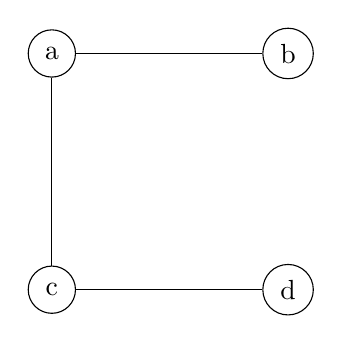
\begin{tikzpicture}[every node/.style={circle,draw,minimum size=6mm}]
  \node (a) {a};
  \node (b) [right of=a,xshift=2cm] {b};
  \node (c) [below of=a,yshift=-2cm] {c};
  \node (d) [below of=b,yshift=-2cm] {d};
  \draw (a)--(b);
  \draw (a)--(c);
  \draw (c)--(d);
\end{tikzpicture}
\end{center}

\section{Forest}
A \textbf{Forest} is a set of trees.

\begin{center}
\begin{tikzpicture}[every node/.style={circle,draw,minimum size=6mm}]
  % Tree 1
  \node (a) {a};
  \node (b) [below of=a,yshift=-1cm] {b};
  \draw (a)--(b);
  % Tree 2
  \node (c) [right of=a,xshift=4cm] {c};
  \node (d) [below of=c,yshift=-1cm] {d};
  \node (e) [below of=d,yshift=-1cm] {e};
  \draw (c)--(d)--(e);
\end{tikzpicture}
\end{center}

\end{document}
